\documentclass[10pt,letterpaper]{article}
\usepackage[top=0.85in,left=2.75in,footskip=0.75in]{geometry}


\usepackage{amsmath,amssymb}
\usepackage{changepage}
\usepackage{textcomp,marvosym}
\usepackage{cite}
\usepackage{nameref,hyperref}
\usepackage[right]{lineno}
\usepackage[nopatch=eqnum]{microtype}
\DisableLigatures[f]{encoding = *, family = * }
\usepackage[table]{xcolor}
\usepackage{array}
\newcolumntype{+}{!{\vrule width 2pt}}
\newlength\savedwidth
\newcommand\thickcline[1]{%
	\noalign{\global\savedwidth\arrayrulewidth\global\arrayrulewidth 2pt}%
	\cline{#1}%
	\noalign{\vskip\arrayrulewidth}%
	\noalign{\global\arrayrulewidth\savedwidth}%
}
\newcommand\thickhline{\noalign{\global\savedwidth\arrayrulewidth\global\arrayrulewidth 2pt}%
	\hline
	\noalign{\global\arrayrulewidth\savedwidth}}

\usepackage{setspace} 
\doublespacing
\raggedright
\setlength{\parindent}{0.5cm}
\textwidth 5.25in 
\textheight 8.75in
\usepackage[aboveskip=1pt,labelfont=bf,labelsep=period,justification=raggedright,singlelinecheck=off]{caption}
\renewcommand{\figurename}{Fig}
\bibliographystyle{unsrt}



% Header and Footer with logo
\usepackage{lastpage,fancyhdr,graphicx}
\usepackage{epstopdf}
%\pagestyle{myheadings}
\pagestyle{fancy}
\fancyhf{}
%\setlength{\headheight}{27.023pt}
%\lhead{\includegraphics[width=2.0in]{PLOS-submission.eps}}
\rfoot{\thepage/\pageref{LastPage}}
\renewcommand{\headrulewidth}{0pt}
\renewcommand{\footrule}{\hrule height 2pt \vspace{2mm}}
\fancyheadoffset[L]{2.25in}
\fancyfootoffset[L]{2.25in}
\lfoot{\today}

%% Include all macros below

\newcommand{\lorem}{{\bf LOREM}}
\newcommand{\ipsum}{{\bf IPSUM}}

%% END MACROS SECTION


\begin{document}
	\vspace*{0.2in}
	
	% Title must be 250 characters or less.
	\begin{flushleft}
		{\Large
			\textbf\newline{Determinants and spatio-temporal structure of SARS-CoV-2 viral load in wastewater in Switzerland: key insights for future surveillance efforts} 
		}
		\newline
		% Insert author names, affiliations and corresponding author email (do not include titles, positions, or degrees).
		\\
		
		Julien Riou\textsuperscript{1\textcurrency*}, 
		People from EAWAG? (Tim, Christoph...),
		People from BAG? (Rita, Anna, Moritz...),
		People from ETHZ? (James, Tanja...),
		\\
		\bigskip
		\textbf{1} Department of Epidemiology and Health Systems, Unisanté, Center for Primary Care and Public Health \& University of Lausanne, Lausanne, Switzerland
		\\
		\textbf{2} 
		\\
		
		\bigskip
		\Yinyang These authors contributed equally to this work.
		
		\textcurrency Current Address: Route de la corniche 10, CH-1010 Lausanne, Switzerland
		
		*Current email: julien.riou@unisante.ch
		
	\end{flushleft}

\section*{Abstract}



\linenumbers

\section{Introduction}

Wastewater-based epidemiology (WBE) has now taken a central role in infectious disease surveillance.
While the analysis of wastewater concentrations of drugs, pharmaceuticals, and other biomarkers at wastewater treatment plants (WWTPs) has been used for decades, the application of this method to assess the epidemiology of pathogens within communities (besides enteric bacteria) is a fairly recent development\cite{choiWastewaterbasedEpidemiologyBiomarkers2018a}, fueled by the increased needs for surveillance during the SARS-CoV-2 pandemic.
WBE is now being used in at least 34 countries\cite{shahWastewaterSurveillanceInfer2022}.
This increase in popularity can be explained by several factors. 
As opposed to diagnosis-based approaches based on the notification of cases, hospitalizations and deaths with a positive laboratory test, WBE can be considered as a population-based approach that does not depend on testing, which is itself influenced by age, gender, and socio-economic position\cite{scullySexGenderDifferences2021,stallSexAgeSpecificDifferences2020,riouSocioeconomicPositionCOVID192021}.
Because it is exempt from testing bias, WBE can be considered as more representative of the entirety of the population living in the WWTP catchment areas, including people with no or mild symptoms, and people less likely to seek care with a health professional. 
WBE is also less costly and less intrusive than individual testing, and can be obtained in near real-time.
However, its full potential and limitations are still being explored.

WBE relies upon the repeated collection of wastewater samples in a generally fixed set of WWTPs.
For SARS-CoV-2, either quantitative Polymerase Chain Reaction (qPCR) or digital droplet PCR (dPCR) tests are then applied to obtain measurements of viral RNA concentrations (generally expressed in gene copies [gc] per liter).  
These measurements are then scaled based on the population living in the WWTP catchment area and on the flow of wastewater on the same day, resulting in a quantity called \textit{viral load} (expressed in gc per day per 100,000 population).
This normalization, by allowing for comparisons over time and space, is key in the use of these data to assess the dynamics of infection at the population level\cite{kirbyUsingWastewaterSurveillance2021,bovenPatternsSARSCoV2Circulation2023,naughtonShowUsData2023}, and also allows for the computation of reproduction numbers\cite{huismanWastewaterBasedEstimationEffective2022}.
But a deeper look into the mechanisms of generation of wastewater data reveals many uncertainties in the pathway leading from  population prevalence to viral load.
First, fecal shedding upon infection with SARS-CoV-2 dominates shedding routes into community-level wastewater, and is also highly heterogeneous.
The probability of fecal shedding is about 40-50\% on average, but is higher in case of gastro-intestinal symptoms\cite{zhangPrevalencePersistentShedding2021,natarajanGastrointestinalSymptomsFecal2022}.
Fecal shedding lasts longer in symptomatic infections compared to asymptomatic, and in adults compared to children\cite{yanCharacteristicsViralShedding2021}.
Virus titre in faeces can also vary widely according to individual characteristics\cite{foladoriSARSCoV2FaecesWastewater2020}.
Second, the population residing within WWTP catchment areas is not as well-defined as generally considered, with movements during the day due to commuting and work, and periodic changes within weeks and years depending on holiday periods.
A third source of variability may be different laboratory methods (e.g., targeting N or S proteins) and protocols (e.g., RNA degradation over time until testing) that can influence measured values\cite{foladoriSARSCoV2FaecesWastewater2020}.
A direct consequence of these observations is that wastewater viral load data may suffer from increased levels of noise and bias depending on the local situation.

In this study, we take advantage of the dense network of WWTPs participating in SARS-CoV-2 surveillance in Switzerland to disentangle the different sources of variability and bias, and characterize the local determinants and the space-time structure of measured SARS-CoV-2 viral load. 
We then use these insights to produce adjusted temporal trends at the national and regional levels, corresponding to the underlying dynamics of SARS-CoV-2 infection after removing all other known sources of variability and bias.
We also consider the spatial structure of the data using clustering techniques, allowing to identify areas with similar profiles.

\section{Methods}

\subsection{Data}

\subsubsection{Viral concentration in wastewater}

This work is based on wastewater samples collected between 7 February 2022 and 21 November 2023 in WWTPs participating to the wastewater surveillance programme coordinated by the Swiss Federal Institute of Aquatic Science and Technology (EAWAG) and the Federal Office of Public Health (FOPH).
A total of 118 WWTPs covering all 26 cantons participated in the programme at least once, including 6 WWTPs directly overseen by EAWAG (with an internal laboratory) that participated for the whole period (Table \ref{tab_desc}).
The minimal length of participation for a WWTP was 106 days.
The frequency of sampling varied between 1.7 and 6.5 times per week on average depending on the WWTP.
Samples were stored on site at 4$^o$C and transported in batches to 9 different laboratories for testing.
Laboratories used slightly different methods for concentration, extraction and quantification with qPCR/dPCR, and two laboratories changed their method during the study period.
Measurements below the limit of quantification (LOQ) and below the limit of detection (LOD) were flagged as such.
The flow of wastewater on the day of the sampling was also measured, and used for normalization.
More details about the processing can be found elsewhere\cite{nadeauInfluenzaTransmissionDynamics2024}.

\subsubsection{Local data}

We used publicly available datasets from the Federal Statistical Office (FSO) to produce variables at the level of the WWTP catchment area.
These included the total resident population by hectare, the resident population under 20 and over 65 by hectare, resident population without Swiss or EU nationality by hectare, and the Swiss index of socio-economic position (SEP) by building.
We aggregated these data using the geographical shapes of WWTP catchment areas developed at FOPH/EAWAG based on the local sewer systems (I also remember something about BAFU)?.


\subsubsection{Data analysis}

Measurements of viral concentration ($C$, unit: gene copies [gc] per liter) were transformed into viral load ($V$; unit: gc per day per 100,000) using the flow of wastewater on the same day ($F$) and the size of the population of the WWTP catchment area ($P$):
$$
  V = \frac{C \times F}{P/100,000}.
$$


\begin{table}[h]
	\centering
	\caption{Description of wastewater data used for SARS-CoV-2 surveillance in Switzerland (2022-2023).}
	\label{tab_desc}
	\scalebox{.9}{\begin{tabular}{ll}
		\hline
		& Value (count or median and range) \\ 
		\hline
		Number of WWTPs & 118 \\ 
		Number of laboratories & 9 \\ 
		Number of laboratory methods & 11 \\ 
		Total measurements & 23,025 \\ 
		Measurements below LOQ & 675 \\ 
		Measurements below LOD & 110 \\ 
		Date of first measurement & 2022-02-07 \\ 
		Date of last measurement & 2023-11-21 \\ 
		Viral concentration [gc/L] & 94,350 (range: 0 to 18,162,400) \\ 
		Wastewater flow [m3/day] & 14,343 (range: 291 to 913,343) \\ 
		Viral load [gc/day/100,000] & 3.7e+12 (range: 1.0e+00 to 7.4e+14) \\ 
		Population covered & 37,507 (range: 2,095 to 475,198) \\ 
		Proportion of population under 20 & 0.24 (range: 0.18 to 0.35) \\ 
		Proportion of population over 65 & 0.36 (range: 0.22 to 0.69) \\ 
		Proportion of population non-Swiss & 0.15 (range: 0.05 to 0.30) \\ 
		Median of Swiss index of socio-economic position (SEP) & 63 (range: 54 to 78) \\ 
		\hline
	\end{tabular}}
\end{table}

\section{Results}

\subsection{Description, table, maps (TBR)}

\begin{figure}[b]
	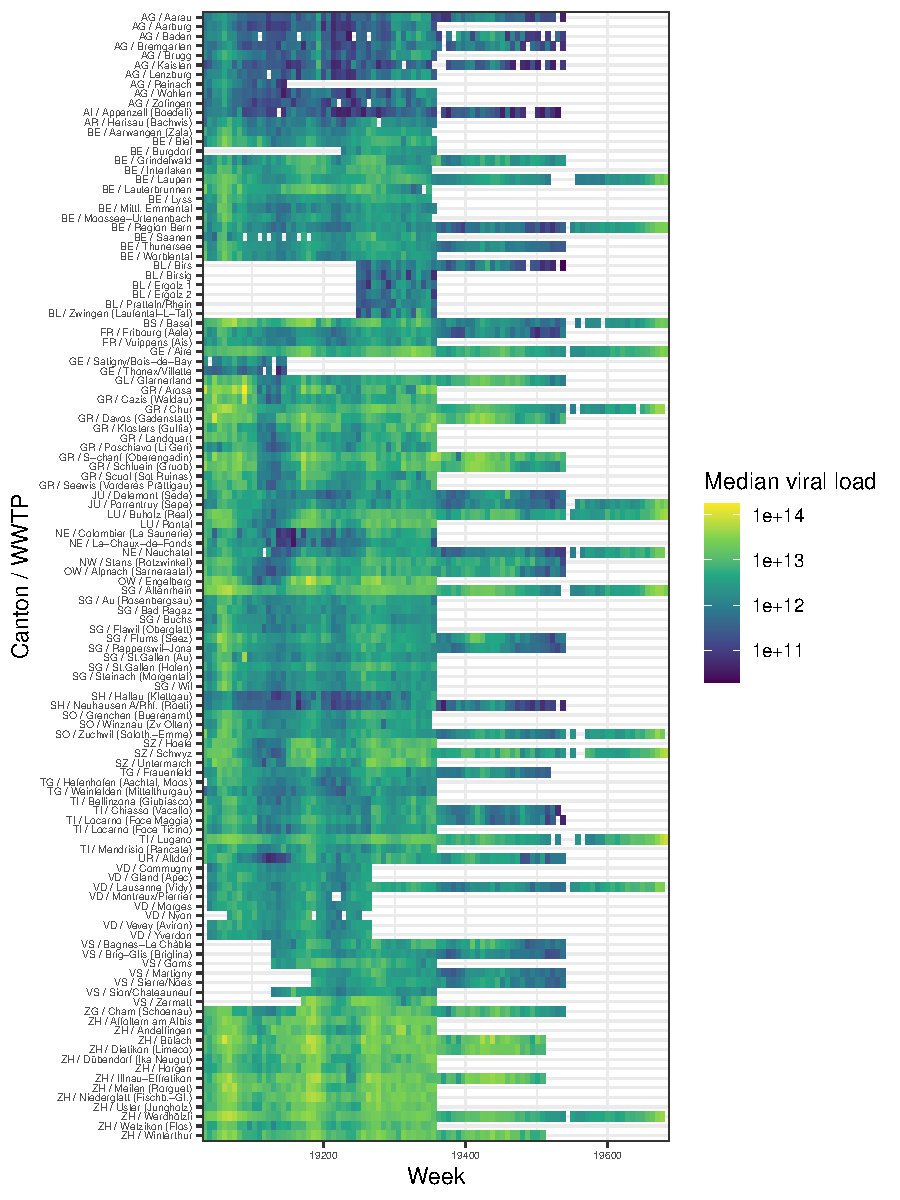
\includegraphics[width=\linewidth]{figures/fig1b.pdf}
	\caption{Weekly median SARS-CoV-2 viral load in wastewater by wastewater treatment plant [WWTP] (values below the limit of detection or of quantification are removed). }
	\label{fig_desc}
\end{figure}

\subsection{local determinants (TBR)}

\subsection{spatial structure (TBR)}

\subsection{single temporal trend (TBR)}

\subsection{spatial clustering (TBR)}

\section{Discussion}

Focus on old, symptomatic is actually an advantage if you want to anticipate on the burden



\nolinenumbers

\section*{Supporting information}


\paragraph*{S1 Text.}
\label{supp1}
{\bf .}


\section*{Acknowledgments}

We gratefully acknowledge all data contributors...


\section*{Funding}


\section*{Data and Code Availability}


\bibliography{wastewater}

\end{document}
